\section{\ref{PS:Q:Scalability}}

\textit{How will the new decentralized solution influence regulation time of a single regulations cycle compared to the current Siemens system?}

\subsection{Experiment}
\label{subsec:Exper:Scale}
Question \ref{PS:Q:Scalability} of \cref{sec:problemStatement} asks how the proposed decentralized system compares to the existing centralized system\cref{cha:existingSystem}) at Siemens Wind Power with regards to a number of parameters.
The experiments below aims to show how the number of turbines and regulation speed affect the regulation algorithm, memory consumption and Network traffic.
Each of these parameters behave differently when centralized compared to decentralized as seen in \cref{fig:timingCentralVSDecentral} the decentralized system does not wait for new data before doing calculations. Because of this the proposed decentralized version has a extra parameter which indicate how much data was updated before the calculation started.

\begin{figure}[b]
	%The figure show how regulation time differs central vs decantral
	\centering
	{\sffamily{Centralized approach}}
	\newline
	

{ %The brackets issolate the enviroment

\makeatletter
\ifcsname c@wavenum\endcsname %Only create one counter
\else
	\newcounter{wavenum}
\fi
\makeatother

\newcommand*{\bitvector}[3]{
  \draw[fill=#3] (t_cur) -- ++( .1, .3) -- ++(#2-.2,0) -- ++(.1, -.3)
                         -- ++(-.1,-.3) -- ++(.2-#2,0) -- cycle;
  \path (t_cur) -- node[anchor=mid] {#1} ++(#2,0) node[time] (t_cur) {};
}

% \known{val}{length}
\newcommand*{\known}[2]{
    \bitvector{#1}{#2}{white}
}

% \unknown{length}
\newcommand*{\unknown}[2]{
    \bitvector{#1}{#2}{black!20}
}

% \nextwave{name}
\newcommand{\nextwave}[1]{
  \path (0,\value{wavenum}) node[left] {#1} node[time] (t_cur) {};
  \addtocounter{wavenum}{-1}
}

% \begin{wave}[clkname]{num_waves}{clock_cycles}
\newenvironment{wave}{
  \begin{tikzpicture}[draw=black, yscale=.8,xscale=1]
    \tikzstyle{time}=[coordinate]
    \setlength{\unitlength}{1cm}
    \setcounter{wavenum}{0}
    
}{\end{tikzpicture}}

%%% End of timing.sty

\begin{wave}
 \nextwave{Regulation Time} \unknown{SendData}{2} \known{WaitForData}{5} \unknown{ReciveData}{2} \unknown{Calculate}{2}
\end{wave}
}

	\newline
	
	{\sffamily{Decentralized approach with seperate data reception}}
	

{ %The brackets issolate the enviroment

\makeatletter
\ifcsname c@wavenum\endcsname %Only create one counter
\else
	\newcounter{wavenum}
\fi
\makeatother

\newcommand*{\bitvector}[3]{
  \draw[fill=#3] (t_cur) -- ++( .1, .3) -- ++(#2-.2,0) -- ++(.1, -.3)
                         -- ++(-.1,-.3) -- ++(.2-#2,0) -- cycle;
  \path (t_cur) -- node[anchor=mid](textNode) {#1} ++(#2,0) node[time] (t_cur) {};
}

% \known{val}{length}
\newcommand*{\known}[2]{
    \bitvector{#1}{#2}{white}
}

% \unknown{length}
\newcommand*{\unknown}[2]{
    \bitvector{#1}{#2}{black!20}
}

% \nextwave{name}
\newcommand{\nextwave}[1]{
  %\path (0,\value{wavenum}) node[left] {#1} node[time] (t_cur) {};
  \path (0,\value{wavenum}) node[time] (t_cur) {};
  \addtocounter{wavenum}{-1}
}

%\newcommand{\timeSpanLabel}{
%	\node (CycleTimeLabel) [rectangle, above = 0.25cm of textNode, inner sep=10pt] {CycleTime};	  
%}

\newcommand{\timeSpanLabel}{
	\node (CycleTimeLabel) [rectangle, above = 1.02cm of t_cur, inner sep=0pt] {Regulation cycle time};
}

\newcommand{\timeSpanA}{
	\node (t_timeSpanA) [point, above = 0 of t_cur] {};	  
}

\newcommand{\timeSpanB}{
	\node (t_timeSpanB) [point, above =0 of t_cur] {};
	
	\graph[use existing nodes]{
		t_timeSpanA --[time span=1cm] CycleTimeLabel;
		CycleTimeLabel.south --[time span=-0.24cm] t_timeSpanB;
	}; 
	
}

%%% End of timing.sty

\begin{tikzpicture}[
	point/.style={inner sep=0pt}, %circle,minimum size=2pt,fill=red},
	draw=black, 
	yscale=.8,
	xscale=1,
	hv path/.style={to path={-| (\tikztotarget)}},
	vh path/.style={to path={|- (\tikztotarget)}},
	skip loop v/.style={to path={-- ++(#1,0) |- (\tikztotarget)}},		
	skip loop h/.style={to path={-- ++(0,#1) -| (\tikztotarget)}},
	time span/.style={to path={-- ++(0,#1) -| (\tikztotarget)}},
	graphs/every graph/.style={edges=rounded corners}	
]
	
\tikzstyle{time}=[coordinate]
\setlength{\unitlength}{1cm}
\setcounter{wavenum}{0}

	\nextwave{} \timeSpanA \unknown{readStates}{3} \unknown{calculate}{3} \timeSpanLabel \unknown{setSetpoint}{3} \unknown{sendState}{3} \timeSpanB \known{wait}{2}
	\nextwave{} \known{reciveStates}{14}
\end{tikzpicture}
}

	\caption{Centralized vs decentralized regulation time}
	\label{fig:timingCentralVSDecentral}
\end{figure}

	The centralized version is split into two applications a client and a server.
	The aim is to compare the regulation time, therefore the client side of the application is not measured. This means that the decentralized version is at a slight disadvantage.
	The following procedure is used each time the experiment is done, the procedure is done with N simulated turbines for both :

\begin{minipage}{\textwidth}
	\begin{enumerate}
		\item Start the system with N turbines.
		\item Make sure the system is stable.
		\item Start logging:
		\begin{itemize}
			\item Reported regulation run time (Central only, Decentralized is reused)
			\item Memory and Bandwidth
		\end{itemize}
		\item Stop logging after \experiemntRunTime.
		\end{enumerate}
\end{minipage}


\subsection{Results}

\begin{figure}[h!]
	\centering
%	\begin{tikzpicture}
\begin{axis}
[
	width=\resultsPlotWidthScale\textwidth,
	axis y line*=left,
	xlabel=Number of turbines,
	ylabel=Regulation cycle time (ms),
	ymin = 0,
	xmin = 1, xmax = 20,
	xtick={1, 2, 3, 4, 5, 6, 7, 8, 9, 10, 11, 12, 13, 14, 15, 16, 17, 18, 19},
	xticklabels={ , , 15, , 25, , 35, , 45, , 55, , 65, , 75, , 85, , 95},
%	xticklabels={5, 10, 15, 20, 25, 30, 35, 40, 45, 50, 55, 60, 65, 70, 75, 80, 85, 90, 95},
	boxplot/draw direction=y,
	ymajorgrids=true,
	yminorgrids=true,
%	minor y tick num=1,
	max space between ticks=17.5
]

%% /home/stefan/work/TestResults/Test4_Centralized_success_12-4-2014_2024/CentralizedLog2.csv
%\buildBoxPlot{0.871522}{0.955}{0.809034}{12.535623}{0.541744}
\buildBoxPlot[black]{0}{0}{0}{0}{0}

%% /home/stefan/work/TestResults/Test4_Centralized_success_12-4-2014_2024/CentralizedLog3.csv
\buildBoxPlot{1.168815}{1.310873}{1.081427}{24.566027}{0.591135}

%% /home/stefan/work/TestResults/Test4_Centralized_success_12-4-2014_2024/CentralizedLog4.csv
\buildBoxPlot{1.398871}{1.613768}{1.303639}{19.188073}{0.747894}

%% /home/stefan/work/TestResults/Test4_Centralized_success_12-4-2014_2024/CentralizedLog5.csv
\buildBoxPlot{1.722236}{1.981776}{1.596331}{13.257023}{1.077214}

%% /home/stefan/work/TestResults/Test4_Centralized_success_12-4-2014_2024/CentralizedLog6.csv
\buildBoxPlot{1.978881}{2.337657}{1.823133}{20.243534}{1.278172}

%% /home/stefan/work/TestResults/Test4_Centralized_success_12-4-2014_2024/CentralizedLog7.csv
\buildBoxPlot{2.985681}{3.527133}{2.724617}{102.89112}{1.917354}

%% /home/stefan/work/TestResults/Test4_Centralized_success_12-4-2014_2024/CentralizedLog8.csv
\buildBoxPlot{5.662268}{6.776311}{5.315074}{55.800126}{3.845115}

%% /home/stefan/work/TestResults/Test4_Centralized_success_12-4-2014_2024/CentralizedLog9.csv
\buildBoxPlot{14.607313}{22.842589}{10.21933}{40.119104}{7.578863}

%% /home/stefan/work/TestResults/Test4_Centralized_success_12-4-2014_2024/CentralizedLog10.csv
\buildBoxPlot{16.673738}{25.382756}{14.810635}{46.844742}{12.042462}

%% /home/stefan/work/TestResults/Test4_Centralized_success_12-4-2014_2024/CentralizedLog11.csv
\buildBoxPlot{20.220936}{27.962488}{19.190067}{63.348974}{17.058657}

%% /home/stefan/work/TestResults/Test4_Centralized_success_12-4-2014_2024/CentralizedLog12.csv
\buildBoxPlot{31.587407}{33.177592}{24.950794}{46.841843}{22.941051}

%% /home/stefan/work/TestResults/Test4_Centralized_success_12-4-2014_2024/CentralizedLog13.csv
\buildBoxPlot{36.93711}{38.790125}{32.230331}{51.398495}{29.702809}

%% /home/stefan/work/TestResults/Test4_Centralized_success_12-4-2014_2024/CentralizedLog14.csv
\buildBoxPlot{40.231022}{42.885333}{36.673407}{77.051599}{33.854906}

%% /home/stefan/work/TestResults/Test4_Centralized_success_12-4-2014_2024/CentralizedLog15.csv
\buildBoxPlot{45.380062}{48.694656}{42.841453}{225.894089}{39.402015}

%% /home/stefan/work/TestResults/Test4_Centralized_success_12-4-2014_2024/CentralizedLog16.csv
\buildBoxPlot{51.425649}{54.462315}{48.438981}{250.200229}{45.062697}

%% /home/stefan/work/TestResults/Test4_Centralized_success_12-4-2014_2024/CentralizedLog17.csv
\buildBoxPlot{58.196177}{62.557505}{55.582236}{271.626595}{51.598593}

%% /home/stefan/work/TestResults/Test4_Centralized_success_12-4-2014_2024/CentralizedLog18.csv
\buildBoxPlot{64.70376}{70.553035}{62.053219}{278.866888}{57.401402}

%% /home/stefan/work/TestResults/Test4_Centralized_success_12-4-2014_2024/CentralizedLog19.csv
\buildBoxPlot{73.715686}{80.566923}{69.809765}{287.542878}{65.698499}

%% /home/stefan/work/TestResults/Test4_Centralized_success_12-4-2014_2024/CentralizedLog20.csv
\buildBoxPlot{82.961949}{151.608592}{77.825807}{290.243704}{72.589561}


\addplot[thick, red!70] coordinates {
%	(1 ,0.871522)
	(2 ,1.168815)
	(3 ,1.398871)
	(4 ,1.722236)
	(5 ,1.978881)
	(6 ,2.985681)
	(7 ,5.662268)
	(8 ,14.607313)
	(9 ,16.673738)
	(10 ,20.220936)
	(11 ,31.587407)
	(12 ,36.93711)
	(13 ,40.231022)
	(14 ,45.380062)
	(15 ,51.425649)
	(16 ,58.196177)
	(17 ,64.70376)
	(18 ,73.715686)
	(19 ,82.961949)
};

\end{axis}
\end{tikzpicture}

	% This file was created by matlab2tikz.
% Minimal pgfplots version: 1.3
%
%The latest updates can be retrieved from
%  http://www.mathworks.com/matlabcentral/fileexchange/22022-matlab2tikz
%where you can also make suggestions and rate matlab2tikz.
%
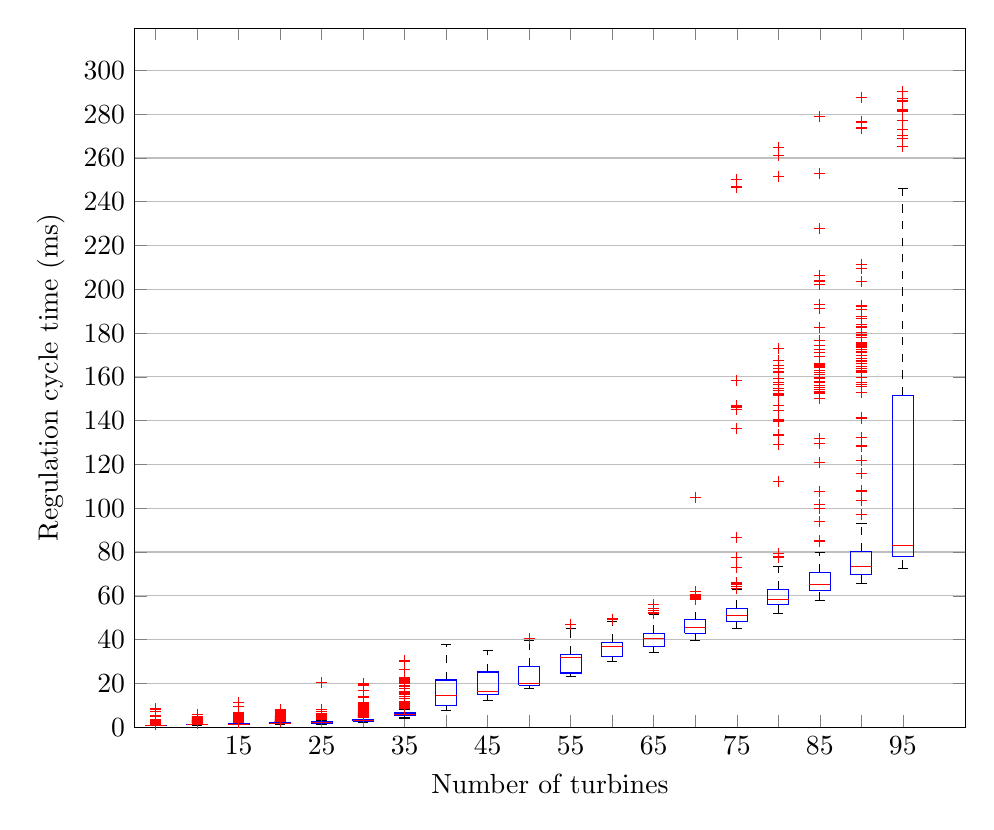
\begin{tikzpicture}

\begin{axis}[%
	width=\resultsPlotWidthScale\textwidth,
	xmin=0.5,
	xmax=20.5,
	xlabel=Number of turbines,
	ylabel=Regulation cycle time (ms),
	xtick={1, 2, 3, 4, 5, 6, 7, 8, 9, 10, 11, 12, 13, 14, 15, 16, 17, 18, 19},
	xticklabels={ , , 15, , 25, , 35, , 45, , 55, , 65, , 75, , 85, , 95},
	ymin=0,
%	ymax=300,
	ymajorgrids=true,
	yminorgrids=true,
	max space between ticks=17.5
]
\addplot [color=black,dashed,forget plot]
  table[row sep=crcr]{%
1	0.955499\\
1	1.156637\\
};
\addplot [color=black,dashed,forget plot]
  table[row sep=crcr]{%
2	1.370008\\
2	1.786582\\
};
\addplot [color=black,dashed,forget plot]
  table[row sep=crcr]{%
3	1.673373\\
3	2.174249\\
};
\addplot [color=black,dashed,forget plot]
  table[row sep=crcr]{%
4	1.958627\\
4	2.487973\\
};
\addplot [color=black,dashed,forget plot]
  table[row sep=crcr]{%
5	2.424964\\
5	3.23762\\
};
\addplot [color=black,dashed,forget plot]
  table[row sep=crcr]{%
6	3.359207\\
6	4.343135\\
};
\addplot [color=black,dashed,forget plot]
  table[row sep=crcr]{%
7	6.472311\\
7	8.243171\\
};
\addplot [color=black,dashed,forget plot]
  table[row sep=crcr]{%
8	21.564196\\
8	37.584364\\
};
\addplot [color=black,dashed,forget plot]
  table[row sep=crcr]{%
9	25.210282\\
9	34.938512\\
};
\addplot [color=black,dashed,forget plot]
  table[row sep=crcr]{%
10	27.678968\\
10	39.521324\\
};
\addplot [color=black,dashed,forget plot]
  table[row sep=crcr]{%
11	33.133063\\
11	45.066276\\
};
\addplot [color=black,dashed,forget plot]
  table[row sep=crcr]{%
12	38.659741\\
12	48.386618\\
};
\addplot [color=black,dashed,forget plot]
  table[row sep=crcr]{%
13	42.692349\\
13	51.64833\\
};
\addplot [color=black,dashed,forget plot]
  table[row sep=crcr]{%
14	48.995592\\
14	58.222076\\
};
\addplot [color=black,dashed,forget plot]
  table[row sep=crcr]{%
15	54.185768\\
15	62.996037\\
};
\addplot [color=black,dashed,forget plot]
  table[row sep=crcr]{%
16	62.88196\\
16	73.366361\\
};
\addplot [color=black,dashed,forget plot]
  table[row sep=crcr]{%
17	70.609667\\
17	79.750216\\
};
\addplot [color=black,dashed,forget plot]
  table[row sep=crcr]{%
18	80.203607\\
18	93.075175\\
};
\addplot [color=black,dashed,forget plot]
  table[row sep=crcr]{%
19	151.608592\\
19	246.076944\\
};
\addplot [color=black,dashed,forget plot]
  table[row sep=crcr]{%
1	0.691463\\
1	0.814662\\
};
\addplot [color=black,dashed,forget plot]
  table[row sep=crcr]{%
2	0.848749\\
2	1.088204\\
};
\addplot [color=black,dashed,forget plot]
  table[row sep=crcr]{%
3	1.082791\\
3	1.330567\\
};
\addplot [color=black,dashed,forget plot]
  table[row sep=crcr]{%
4	1.225531\\
4	1.59823\\
};
\addplot [color=black,dashed,forget plot]
  table[row sep=crcr]{%
5	1.440994\\
5	1.862917\\
};
\addplot [color=black,dashed,forget plot]
  table[row sep=crcr]{%
6	2.148756\\
6	2.694676\\
};
\addplot [color=black,dashed,forget plot]
  table[row sep=crcr]{%
7	4.178016\\
7	5.258074\\
};
\addplot [color=black,dashed,forget plot]
  table[row sep=crcr]{%
8	7.806459\\
8	9.763918\\
};
\addplot [color=black,dashed,forget plot]
  table[row sep=crcr]{%
9	12.116028\\
9	14.873879\\
};
\addplot [color=black,dashed,forget plot]
  table[row sep=crcr]{%
10	17.509834\\
10	19.152298\\
};
\addplot [color=black,dashed,forget plot]
  table[row sep=crcr]{%
11	23.186344\\
11	24.757905\\
};
\addplot [color=black,dashed,forget plot]
  table[row sep=crcr]{%
12	29.984252\\
12	32.129229\\
};
\addplot [color=black,dashed,forget plot]
  table[row sep=crcr]{%
13	33.953182\\
13	36.679471\\
};
\addplot [color=black,dashed,forget plot]
  table[row sep=crcr]{%
14	39.402015\\
14	42.832867\\
};
\addplot [color=black,dashed,forget plot]
  table[row sep=crcr]{%
15	45.162367\\
15	48.235799\\
};
\addplot [color=black,dashed,forget plot]
  table[row sep=crcr]{%
16	51.804628\\
16	55.840494\\
};
\addplot [color=black,dashed,forget plot]
  table[row sep=crcr]{%
17	57.925799\\
17	62.39761\\
};
\addplot [color=black,dashed,forget plot]
  table[row sep=crcr]{%
18	65.7218\\
18	69.72912\\
};
\addplot [color=black,dashed,forget plot]
  table[row sep=crcr]{%
19	72.589561\\
19	77.840082\\
};
\addplot [color=black,solid,forget plot]
  table[row sep=crcr]{%
0.875	1.156637\\
1.125	1.156637\\
};
\addplot [color=black,solid,forget plot]
  table[row sep=crcr]{%
1.875	1.786582\\
2.125	1.786582\\
};
\addplot [color=black,solid,forget plot]
  table[row sep=crcr]{%
2.875	2.174249\\
3.125	2.174249\\
};
\addplot [color=black,solid,forget plot]
  table[row sep=crcr]{%
3.875	2.487973\\
4.125	2.487973\\
};
\addplot [color=black,solid,forget plot]
  table[row sep=crcr]{%
4.875	3.23762\\
5.125	3.23762\\
};
\addplot [color=black,solid,forget plot]
  table[row sep=crcr]{%
5.875	4.343135\\
6.125	4.343135\\
};
\addplot [color=black,solid,forget plot]
  table[row sep=crcr]{%
6.875	8.243171\\
7.125	8.243171\\
};
\addplot [color=black,solid,forget plot]
  table[row sep=crcr]{%
7.875	37.584364\\
8.125	37.584364\\
};
\addplot [color=black,solid,forget plot]
  table[row sep=crcr]{%
8.875	34.938512\\
9.125	34.938512\\
};
\addplot [color=black,solid,forget plot]
  table[row sep=crcr]{%
9.875	39.521324\\
10.125	39.521324\\
};
\addplot [color=black,solid,forget plot]
  table[row sep=crcr]{%
10.875	45.066276\\
11.125	45.066276\\
};
\addplot [color=black,solid,forget plot]
  table[row sep=crcr]{%
11.875	48.386618\\
12.125	48.386618\\
};
\addplot [color=black,solid,forget plot]
  table[row sep=crcr]{%
12.875	51.64833\\
13.125	51.64833\\
};
\addplot [color=black,solid,forget plot]
  table[row sep=crcr]{%
13.875	58.222076\\
14.125	58.222076\\
};
\addplot [color=black,solid,forget plot]
  table[row sep=crcr]{%
14.875	62.996037\\
15.125	62.996037\\
};
\addplot [color=black,solid,forget plot]
  table[row sep=crcr]{%
15.875	73.366361\\
16.125	73.366361\\
};
\addplot [color=black,solid,forget plot]
  table[row sep=crcr]{%
16.875	79.750216\\
17.125	79.750216\\
};
\addplot [color=black,solid,forget plot]
  table[row sep=crcr]{%
17.875	93.075175\\
18.125	93.075175\\
};
\addplot [color=black,solid,forget plot]
  table[row sep=crcr]{%
18.875	246.076944\\
19.125	246.076944\\
};
\addplot [color=black,solid,forget plot]
  table[row sep=crcr]{%
0.875	0.691463\\
1.125	0.691463\\
};
\addplot [color=black,solid,forget plot]
  table[row sep=crcr]{%
1.875	0.848749\\
2.125	0.848749\\
};
\addplot [color=black,solid,forget plot]
  table[row sep=crcr]{%
2.875	1.082791\\
3.125	1.082791\\
};
\addplot [color=black,solid,forget plot]
  table[row sep=crcr]{%
3.875	1.225531\\
4.125	1.225531\\
};
\addplot [color=black,solid,forget plot]
  table[row sep=crcr]{%
4.875	1.440994\\
5.125	1.440994\\
};
\addplot [color=black,solid,forget plot]
  table[row sep=crcr]{%
5.875	2.148756\\
6.125	2.148756\\
};
\addplot [color=black,solid,forget plot]
  table[row sep=crcr]{%
6.875	4.178016\\
7.125	4.178016\\
};
\addplot [color=black,solid,forget plot]
  table[row sep=crcr]{%
7.875	7.806459\\
8.125	7.806459\\
};
\addplot [color=black,solid,forget plot]
  table[row sep=crcr]{%
8.875	12.116028\\
9.125	12.116028\\
};
\addplot [color=black,solid,forget plot]
  table[row sep=crcr]{%
9.875	17.509834\\
10.125	17.509834\\
};
\addplot [color=black,solid,forget plot]
  table[row sep=crcr]{%
10.875	23.186344\\
11.125	23.186344\\
};
\addplot [color=black,solid,forget plot]
  table[row sep=crcr]{%
11.875	29.984252\\
12.125	29.984252\\
};
\addplot [color=black,solid,forget plot]
  table[row sep=crcr]{%
12.875	33.953182\\
13.125	33.953182\\
};
\addplot [color=black,solid,forget plot]
  table[row sep=crcr]{%
13.875	39.402015\\
14.125	39.402015\\
};
\addplot [color=black,solid,forget plot]
  table[row sep=crcr]{%
14.875	45.162367\\
15.125	45.162367\\
};
\addplot [color=black,solid,forget plot]
  table[row sep=crcr]{%
15.875	51.804628\\
16.125	51.804628\\
};
\addplot [color=black,solid,forget plot]
  table[row sep=crcr]{%
16.875	57.925799\\
17.125	57.925799\\
};
\addplot [color=black,solid,forget plot]
  table[row sep=crcr]{%
17.875	65.7218\\
18.125	65.7218\\
};
\addplot [color=black,solid,forget plot]
  table[row sep=crcr]{%
18.875	72.589561\\
19.125	72.589561\\
};
\addplot [color=blue,solid,forget plot]
  table[row sep=crcr]{%
0.75	0.814662\\
0.75	0.955499\\
1.25	0.955499\\
1.25	0.814662\\
0.75	0.814662\\
};
\addplot [color=blue,solid,forget plot]
  table[row sep=crcr]{%
1.75	1.088204\\
1.75	1.370008\\
2.25	1.370008\\
2.25	1.088204\\
1.75	1.088204\\
};
\addplot [color=blue,solid,forget plot]
  table[row sep=crcr]{%
2.75	1.330567\\
2.75	1.673373\\
3.25	1.673373\\
3.25	1.330567\\
2.75	1.330567\\
};
\addplot [color=blue,solid,forget plot]
  table[row sep=crcr]{%
3.75	1.59823\\
3.75	1.958627\\
4.25	1.958627\\
4.25	1.59823\\
3.75	1.59823\\
};
\addplot [color=blue,solid,forget plot]
  table[row sep=crcr]{%
4.75	1.862917\\
4.75	2.424964\\
5.25	2.424964\\
5.25	1.862917\\
4.75	1.862917\\
};
\addplot [color=blue,solid,forget plot]
  table[row sep=crcr]{%
5.75	2.694676\\
5.75	3.359207\\
6.25	3.359207\\
6.25	2.694676\\
5.75	2.694676\\
};
\addplot [color=blue,solid,forget plot]
  table[row sep=crcr]{%
6.75	5.258074\\
6.75	6.472311\\
7.25	6.472311\\
7.25	5.258074\\
6.75	5.258074\\
};
\addplot [color=blue,solid,forget plot]
  table[row sep=crcr]{%
7.75	9.763918\\
7.75	21.564196\\
8.25	21.564196\\
8.25	9.763918\\
7.75	9.763918\\
};
\addplot [color=blue,solid,forget plot]
  table[row sep=crcr]{%
8.75	14.873879\\
8.75	25.210282\\
9.25	25.210282\\
9.25	14.873879\\
8.75	14.873879\\
};
\addplot [color=blue,solid,forget plot]
  table[row sep=crcr]{%
9.75	19.152298\\
9.75	27.678968\\
10.25	27.678968\\
10.25	19.152298\\
9.75	19.152298\\
};
\addplot [color=blue,solid,forget plot]
  table[row sep=crcr]{%
10.75	24.757905\\
10.75	33.133063\\
11.25	33.133063\\
11.25	24.757905\\
10.75	24.757905\\
};
\addplot [color=blue,solid,forget plot]
  table[row sep=crcr]{%
11.75	32.129229\\
11.75	38.659741\\
12.25	38.659741\\
12.25	32.129229\\
11.75	32.129229\\
};
\addplot [color=blue,solid,forget plot]
  table[row sep=crcr]{%
12.75	36.679471\\
12.75	42.692349\\
13.25	42.692349\\
13.25	36.679471\\
12.75	36.679471\\
};
\addplot [color=blue,solid,forget plot]
  table[row sep=crcr]{%
13.75	42.832867\\
13.75	48.995592\\
14.25	48.995592\\
14.25	42.832867\\
13.75	42.832867\\
};
\addplot [color=blue,solid,forget plot]
  table[row sep=crcr]{%
14.75	48.235799\\
14.75	54.185768\\
15.25	54.185768\\
15.25	48.235799\\
14.75	48.235799\\
};
\addplot [color=blue,solid,forget plot]
  table[row sep=crcr]{%
15.75	55.840494\\
15.75	62.88196\\
16.25	62.88196\\
16.25	55.840494\\
15.75	55.840494\\
};
\addplot [color=blue,solid,forget plot]
  table[row sep=crcr]{%
16.75	62.39761\\
16.75	70.609667\\
17.25	70.609667\\
17.25	62.39761\\
16.75	62.39761\\
};
\addplot [color=blue,solid,forget plot]
  table[row sep=crcr]{%
17.75	69.72912\\
17.75	80.203607\\
18.25	80.203607\\
18.25	69.72912\\
17.75	69.72912\\
};
\addplot [color=blue,solid,forget plot]
  table[row sep=crcr]{%
18.75	77.840082\\
18.75	151.608592\\
19.25	151.608592\\
19.25	77.840082\\
18.75	77.840082\\
};
\addplot [color=red,solid,forget plot]
  table[row sep=crcr]{%
0.75	0.874626\\
1.25	0.874626\\
};
\addplot [color=red,solid,forget plot]
  table[row sep=crcr]{%
1.75	1.1775345\\
2.25	1.1775345\\
};
\addplot [color=red,solid,forget plot]
  table[row sep=crcr]{%
2.75	1.4201575\\
3.25	1.4201575\\
};
\addplot [color=red,solid,forget plot]
  table[row sep=crcr]{%
3.75	1.716257\\
4.25	1.716257\\
};
\addplot [color=red,solid,forget plot]
  table[row sep=crcr]{%
4.75	1.9973935\\
5.25	1.9973935\\
};
\addplot [color=red,solid,forget plot]
  table[row sep=crcr]{%
5.75	2.903549\\
6.25	2.903549\\
};
\addplot [color=red,solid,forget plot]
  table[row sep=crcr]{%
6.75	5.5932275\\
7.25	5.5932275\\
};
\addplot [color=red,solid,forget plot]
  table[row sep=crcr]{%
7.75	14.5812775\\
8.25	14.5812775\\
};
\addplot [color=red,solid,forget plot]
  table[row sep=crcr]{%
8.75	16.4337625\\
9.25	16.4337625\\
};
\addplot [color=red,solid,forget plot]
  table[row sep=crcr]{%
9.75	20.091426\\
10.25	20.091426\\
};
\addplot [color=red,solid,forget plot]
  table[row sep=crcr]{%
10.75	31.692363\\
11.25	31.692363\\
};
\addplot [color=red,solid,forget plot]
  table[row sep=crcr]{%
11.75	36.8004425\\
12.25	36.8004425\\
};
\addplot [color=red,solid,forget plot]
  table[row sep=crcr]{%
12.75	40.4086135\\
13.25	40.4086135\\
};
\addplot [color=red,solid,forget plot]
  table[row sep=crcr]{%
13.75	45.333356\\
14.25	45.333356\\
};
\addplot [color=red,solid,forget plot]
  table[row sep=crcr]{%
14.75	50.8482875\\
15.25	50.8482875\\
};
\addplot [color=red,solid,forget plot]
  table[row sep=crcr]{%
15.75	58.49032\\
16.25	58.49032\\
};
\addplot [color=red,solid,forget plot]
  table[row sep=crcr]{%
16.75	65.293539\\
17.25	65.293539\\
};
\addplot [color=red,solid,forget plot]
  table[row sep=crcr]{%
17.75	73.479706\\
18.25	73.479706\\
};
\addplot [color=red,solid,forget plot]
  table[row sep=crcr]{%
18.75	82.948313\\
19.25	82.948313\\
};
\addplot [color=blue,only marks,mark=+,mark options={solid,draw=red},forget plot]
  table[row sep=crcr]{%
1	1.176103\\
1	1.178509\\
1	1.193344\\
1	1.20704\\
1	1.214954\\
1	1.221493\\
1	1.245021\\
1	1.316445\\
1	1.327208\\
1	1.524131\\
1	1.524274\\
1	1.543741\\
1	1.902597\\
1	2.169802\\
1	2.307744\\
1	2.476555\\
1	2.709384\\
1	2.981451\\
1	3.140805\\
1	3.283617\\
1	4.963499\\
1	5.363371\\
1	7.190786\\
1	8.30093\\
};
\addplot [color=blue,only marks,mark=+,mark options={solid,draw=red},forget plot]
  table[row sep=crcr]{%
2	1.793523\\
2	1.845619\\
2	1.848076\\
2	1.933673\\
2	1.99282\\
2	2.051408\\
2	2.120934\\
2	2.151493\\
2	2.249679\\
2	2.262758\\
2	2.300418\\
2	2.368791\\
2	2.401617\\
2	2.481835\\
2	2.53602\\
2	2.548682\\
2	2.576888\\
2	2.597632\\
2	2.677461\\
2	2.723364\\
2	2.740618\\
2	2.774466\\
2	2.867248\\
2	2.899936\\
2	2.944661\\
2	2.965056\\
2	2.96526\\
2	2.981629\\
2	3.089347\\
2	3.131373\\
2	3.180755\\
2	3.306036\\
2	3.332826\\
2	3.449926\\
2	3.489132\\
2	3.672439\\
2	3.706892\\
2	3.749078\\
2	3.877362\\
2	4.023028\\
2	4.389004\\
2	4.398121\\
2	4.401876\\
2	4.678904\\
2	4.779742\\
2	4.918733\\
2	5.075662\\
2	5.601809\\
};
\addplot [color=blue,only marks,mark=+,mark options={solid,draw=red},forget plot]
  table[row sep=crcr]{%
3	2.192261\\
3	2.222847\\
3	2.223433\\
3	2.239635\\
3	2.245748\\
3	2.337855\\
3	2.564155\\
3	2.566424\\
3	2.568352\\
3	2.629852\\
3	2.652528\\
3	2.703118\\
3	2.733534\\
3	2.764757\\
3	2.783863\\
3	2.828118\\
3	2.846928\\
3	2.984215\\
3	3.051839\\
3	3.071094\\
3	3.081963\\
3	3.230031\\
3	3.352067\\
3	3.690988\\
3	3.70011\\
3	3.71423\\
3	4.081016\\
3	4.251259\\
3	4.299668\\
3	4.317077\\
3	4.378226\\
3	4.655414\\
3	4.800068\\
3	5.335757\\
3	5.455589\\
3	5.596238\\
3	5.710081\\
3	5.790715\\
3	6.364993\\
3	6.679123\\
3	9.543143\\
3	11.395216\\
};
\addplot [color=blue,only marks,mark=+,mark options={solid,draw=red},forget plot]
  table[row sep=crcr]{%
4	2.503863\\
4	2.506996\\
4	2.518698\\
4	2.519083\\
4	2.524849\\
4	2.538949\\
4	2.539779\\
4	2.543708\\
4	2.590436\\
4	2.612976\\
4	2.624723\\
4	2.639969\\
4	2.692657\\
4	2.701875\\
4	2.702706\\
4	2.776353\\
4	2.834106\\
4	2.874534\\
4	2.903889\\
4	2.921809\\
4	2.947651\\
4	3.016038\\
4	3.18633\\
4	3.256435\\
4	3.289407\\
4	3.470499\\
4	3.523172\\
4	3.573076\\
4	3.614098\\
4	3.621255\\
4	3.757607\\
4	3.911986\\
4	4.033259\\
4	4.073237\\
4	4.338524\\
4	4.399647\\
4	4.630443\\
4	4.664954\\
4	4.779427\\
4	4.906645\\
4	4.925404\\
4	5.040655\\
4	5.079302\\
4	5.373808\\
4	6.030455\\
4	6.328306\\
4	6.626284\\
4	6.999776\\
4	7.221142\\
4	7.451491\\
4	7.916905\\
};
\addplot [color=blue,only marks,mark=+,mark options={solid,draw=red},forget plot]
  table[row sep=crcr]{%
5	3.320071\\
5	3.377586\\
5	3.423061\\
5	3.427332\\
5	3.53449\\
5	3.546939\\
5	3.746197\\
5	3.765826\\
5	3.782267\\
5	3.787644\\
5	3.824862\\
5	3.893861\\
5	3.959252\\
5	4.037436\\
5	4.097061\\
5	4.125631\\
5	4.133696\\
5	4.138075\\
5	4.147994\\
5	4.176374\\
5	4.421668\\
5	4.513637\\
5	4.616056\\
5	4.635814\\
5	4.753148\\
5	5.167944\\
5	5.19975\\
5	5.420932\\
5	5.455067\\
5	5.665121\\
5	5.721665\\
5	5.83401\\
5	5.87468\\
5	5.89412\\
5	5.921696\\
5	6.057049\\
5	6.131888\\
5	6.296973\\
5	6.321923\\
5	6.343328\\
5	7.090603\\
5	8.26168\\
5	20.243534\\
};
\addplot [color=blue,only marks,mark=+,mark options={solid,draw=red},forget plot]
  table[row sep=crcr]{%
6	4.495225\\
6	4.498673\\
6	4.498827\\
6	4.563186\\
6	4.587355\\
6	4.754654\\
6	5.009052\\
6	5.021732\\
6	5.102506\\
6	5.158721\\
6	5.167734\\
6	5.198709\\
6	5.23857\\
6	5.3746\\
6	5.400768\\
6	5.471458\\
6	5.487853\\
6	5.732529\\
6	5.758585\\
6	5.785591\\
6	5.904012\\
6	6.088597\\
6	6.13559\\
6	6.338497\\
6	6.607769\\
6	6.707598\\
6	6.847774\\
6	6.863557\\
6	6.923896\\
6	6.932131\\
6	6.966114\\
6	7.246241\\
6	7.552089\\
6	7.637072\\
6	8.035988\\
6	8.318994\\
6	8.349444\\
6	8.519427\\
6	8.777099\\
6	9.338181\\
6	9.720935\\
6	9.898789\\
6	10.188432\\
6	10.358991\\
6	10.590425\\
6	11.26527\\
6	13.649585\\
6	13.917339\\
6	16.898115\\
6	19.216894\\
6	19.71008\\
};
\addplot [color=blue,only marks,mark=+,mark options={solid,draw=red},forget plot]
  table[row sep=crcr]{%
7	8.35779\\
7	8.415277\\
7	8.473364\\
7	8.504532\\
7	8.506126\\
7	8.519745\\
7	8.553583\\
7	8.5815\\
7	8.663745\\
7	8.678187\\
7	8.683617\\
7	8.78386\\
7	8.849726\\
7	8.950628\\
7	8.987027\\
7	8.992308\\
7	9.120563\\
7	9.207595\\
7	9.23472\\
7	9.345101\\
7	9.398249\\
7	9.423573\\
7	9.439464\\
7	9.486276\\
7	9.521467\\
7	9.580156\\
7	9.590542\\
7	9.629696\\
7	9.657168\\
7	9.679038\\
7	9.768644\\
7	9.773259\\
7	9.820831\\
7	9.965677\\
7	10.269888\\
7	10.302693\\
7	10.323261\\
7	10.420508\\
7	10.88144\\
7	10.912448\\
7	10.912924\\
7	10.922096\\
7	11.006882\\
7	11.222083\\
7	11.30686\\
7	11.547859\\
7	13.009371\\
7	14.092999\\
7	14.86172\\
7	15.293268\\
7	15.773637\\
7	16.071576\\
7	17.524366\\
7	18.635734\\
7	18.86347\\
7	18.884021\\
7	19.925684\\
7	20.211662\\
7	20.368998\\
7	20.490724\\
7	20.838327\\
7	20.957185\\
7	21.053338\\
7	21.479073\\
7	21.720464\\
7	21.952807\\
7	22.450527\\
7	26.466628\\
7	29.810133\\
7	29.924012\\
7	30.656609\\
};
\addplot [color=blue,only marks,mark=+,mark options={solid,draw=red},forget plot]
  table[row sep=crcr]{%
nan	nan\\
};
\addplot [color=blue,only marks,mark=+,mark options={solid,draw=red},forget plot]
  table[row sep=crcr]{%
nan	nan\\
};
\addplot [color=blue,only marks,mark=+,mark options={solid,draw=red},forget plot]
  table[row sep=crcr]{%
10	40.572149\\
};
\addplot [color=blue,only marks,mark=+,mark options={solid,draw=red},forget plot]
  table[row sep=crcr]{%
11	46.841843\\
};
\addplot [color=blue,only marks,mark=+,mark options={solid,draw=red},forget plot]
  table[row sep=crcr]{%
12	49.32547\\
12	49.39728\\
};
\addplot [color=blue,only marks,mark=+,mark options={solid,draw=red},forget plot]
  table[row sep=crcr]{%
13	51.734931\\
13	52.263042\\
13	52.479868\\
13	53.346653\\
13	53.380803\\
13	54.235959\\
13	56.218855\\
};
\addplot [color=blue,only marks,mark=+,mark options={solid,draw=red},forget plot]
  table[row sep=crcr]{%
14	58.24263\\
14	58.359494\\
14	58.779699\\
14	59.255721\\
14	59.797221\\
14	59.956779\\
14	59.989437\\
14	60.023581\\
14	60.358906\\
14	60.684411\\
14	61.858036\\
14	104.953184\\
};
\addplot [color=blue,only marks,mark=+,mark options={solid,draw=red},forget plot]
  table[row sep=crcr]{%
15	63.495834\\
15	64.370846\\
15	65.078212\\
15	65.674834\\
15	65.803883\\
15	65.835327\\
15	66.021914\\
15	66.103339\\
15	73.001122\\
15	77.636315\\
15	86.826142\\
15	136.487634\\
15	145.283402\\
15	146.099428\\
15	146.233285\\
15	146.323243\\
15	146.921872\\
15	158.423312\\
15	246.362832\\
15	246.722952\\
15	250.200229\\
};
\addplot [color=blue,only marks,mark=+,mark options={solid,draw=red},forget plot]
  table[row sep=crcr]{%
16	77.720929\\
16	79.177628\\
16	112.408851\\
16	128.969515\\
16	133.462981\\
16	139.858548\\
16	140.725977\\
16	144.612062\\
16	146.817379\\
16	151.383076\\
16	151.881108\\
16	151.922485\\
16	152.242982\\
16	153.688064\\
16	154.509165\\
16	156.475983\\
16	157.507242\\
16	159.324566\\
16	162.256717\\
16	164.015403\\
16	165.32339\\
16	167.323423\\
16	172.786236\\
16	251.349021\\
16	261.289044\\
16	264.827819\\
};
\addplot [color=blue,only marks,mark=+,mark options={solid,draw=red},forget plot]
  table[row sep=crcr]{%
17	85.033259\\
17	85.168934\\
17	93.984073\\
17	99.985429\\
17	101.754141\\
17	107.502865\\
17	120.708505\\
17	129.533025\\
17	131.685524\\
17	150.07707\\
17	152.531279\\
17	152.848707\\
17	153.515564\\
17	154.184764\\
17	154.425517\\
17	155.223244\\
17	155.325952\\
17	156.040595\\
17	157.51096\\
17	157.745791\\
17	157.763823\\
17	157.78978\\
17	159.313071\\
17	159.792905\\
17	161.075164\\
17	161.182074\\
17	161.201118\\
17	162.147412\\
17	163.084965\\
17	164.144737\\
17	164.432633\\
17	164.531559\\
17	165.276971\\
17	165.915944\\
17	166.24057\\
17	169.122972\\
17	170.956902\\
17	172.574969\\
17	174.203491\\
17	174.230232\\
17	176.682499\\
17	182.438894\\
17	191.366639\\
17	192.967176\\
17	202.370675\\
17	203.807066\\
17	206.229644\\
17	227.845875\\
17	252.720361\\
17	278.866888\\
};
\addplot [color=blue,only marks,mark=+,mark options={solid,draw=red},forget plot]
  table[row sep=crcr]{%
18	97.320739\\
18	103.607594\\
18	107.896473\\
18	116.060945\\
18	121.809576\\
18	128.452211\\
18	132.177856\\
18	141.230189\\
18	152.923783\\
18	155.730984\\
18	156.691553\\
18	157.523825\\
18	159.835414\\
18	159.897403\\
18	161.962464\\
18	162.510937\\
18	162.565594\\
18	163.007536\\
18	163.988911\\
18	164.705291\\
18	165.959133\\
18	167.195639\\
18	167.26318\\
18	167.489415\\
18	167.573509\\
18	168.458682\\
18	169.70467\\
18	171.087881\\
18	171.523672\\
18	171.531448\\
18	171.659207\\
18	172.561978\\
18	172.716008\\
18	173.315331\\
18	173.869469\\
18	174.119127\\
18	174.807872\\
18	175.47089\\
18	178.054177\\
18	178.925643\\
18	179.325541\\
18	180.261783\\
18	182.703061\\
18	183.168246\\
18	183.804264\\
18	186.546645\\
18	187.398376\\
18	190.73619\\
18	192.117568\\
18	192.334748\\
18	192.687149\\
18	203.621105\\
18	209.714732\\
18	211.529157\\
18	273.591922\\
18	274.074762\\
18	276.443283\\
18	287.542878\\
};
\addplot [color=blue,only marks,mark=+,mark options={solid,draw=red},forget plot]
  table[row sep=crcr]{%
19	265.296814\\
19	268.749173\\
19	270.245766\\
19	273.069504\\
19	277.122711\\
19	281.054363\\
19	281.926684\\
19	282.148412\\
19	285.594887\\
19	286.16293\\
19	287.331069\\
19	290.243704\\
};
\node[above, align=center, inner sep=0mm, text=black]
at (axis cs:9.13684210526316,-12,0) {1};
\node[above, align=center, inner sep=0mm, text=black]
at (axis cs:27.4105263157895,-12,0) {2};
\node[above, align=center, inner sep=0mm, text=black]
at (axis cs:45.6842105263158,-12,0) {3};
\node[above, align=center, inner sep=0mm, text=black]
at (axis cs:63.9578947368421,-12,0) {4};
\node[above, align=center, inner sep=0mm, text=black]
at (axis cs:82.2315789473684,-12,0) {5};
\node[above, align=center, inner sep=0mm, text=black]
at (axis cs:100.505263157895,-12,0) {6};
\node[above, align=center, inner sep=0mm, text=black]
at (axis cs:118.778947368421,-12,0) {7};
\node[above, align=center, inner sep=0mm, text=black]
at (axis cs:137.052631578947,-12,0) {8};
\node[above, align=center, inner sep=0mm, text=black]
at (axis cs:155.326315789474,-12,0) {9};
\node[above, align=center, inner sep=0mm, text=black]
at (axis cs:173.6,-12,0) {10};
\node[above, align=center, inner sep=0mm, text=black]
at (axis cs:191.873684210526,-12,0) {11};
\node[above, align=center, inner sep=0mm, text=black]
at (axis cs:210.147368421053,-12,0) {12};
\node[above, align=center, inner sep=0mm, text=black]
at (axis cs:228.421052631579,-12,0) {13};
\node[above, align=center, inner sep=0mm, text=black]
at (axis cs:246.694736842105,-12,0) {14};
\node[above, align=center, inner sep=0mm, text=black]
at (axis cs:264.968421052632,-12,0) {15};
\node[above, align=center, inner sep=0mm, text=black]
at (axis cs:283.242105263158,-12,0) {16};
\node[above, align=center, inner sep=0mm, text=black]
at (axis cs:301.515789473684,-12,0) {17};
\node[above, align=center, inner sep=0mm, text=black]
at (axis cs:319.789473684211,-12,0) {18};
\node[above, align=center, inner sep=0mm, text=black]
at (axis cs:338.063157894737,-12,0) {19};
\end{axis}
\end{tikzpicture}%
	\caption{Centralized solution variable number of turbines experiment 1}
	\label{fig:exp:cen:turbines}
\end{figure}

The \nameref{subsec:Exper:Scale} experiment results are described in this section, these experiments are done against the centralized solution. \Cref{fig:exp:cen:turbines} show the comparison experiment done with the centralized solution. The median values initially are constant, this is from 10 turbines to 30 turbines, from 35 and up the median is linearly increasing.
From 70 Turbines the regulation start to have larger max values which increases linearly as well.





\subsection{Discussion}
\subsubsection{Comparison of the decentralized solution and the centralized solution}
\label{sec:comp:decentralizedVScentralized}
The decentralized solution and the centralized solution is built with a very different architecture. This is reflected in the difference in the way the two solutions scale with the number of turbines. Looking at the figures for regulation cycle time in relation to the number of turbines for the decentralized and the centralized solution respectively we see that the figures reveals different trends. The test results from the centralized solution presented in \cref{fig:exp:cen:turbines} shows how adding turbines increases the regulation cycle time. From 5 to 30 turbines the regulation time of the centralized solution increase slowly. After 35 turbines the increase in regulation cycle time becomes steeper. For every 15 turbines added the regulation cycle time increases with approximately $25 ms$. The relation between regulation cycle time and the number of turbines is caused by the direct impact the number of turbines have on the regulation cycle. The Park Pilot of the centralized solution must use additional time on querying each added turbine as well as wait for their individual reply before performing the regulation algorithm. Thus the scalability of the centralized solution is linear with a factor of $25 / 15 = 1.667$.

The scalability of the decentralized solution, as described in \cref{sec:disc:turbinesVScycletime}, is small enough that it is indistinguishable from other factors in our test data and therefore we cannot calculate it. Thus the scalability of the decentralized solution is close to constant. This great improvement in scalability comes with a trade off in terms of cache reads. Adding additional turbines to the decentralized solution the number of cache reads increases with a factor of $0.033$ which is still an improvement compared to the scale factor of the centralized solution. Arguably comparing the scalability of the number of cache reads in the decentralized solution with the scalability of the regulation cycle in the centralized solution is not a viable way to compare the scalability of the two solutions, but comparing the scalability of the regulation cycle of both solutions will not be a fair comparison either since the improvements in scalability of the decentralized solution comes at the price of increased numbers of cache reads.

\subsubsection{Comparison of the decentralized solution and the current Siemens system}
This section address the \ref{PS:Q:Scalability} problem of \cref{sec:problemStatement}.
Comparing the decentralized solution and the current Siemens system directly is impossible given the differences in environment and architecture. Introducing a centralized solution is an attempt to bridge this gap. By comparing the decentralized solution to the centralized solution and measuring the improvements/demotions we can transfer these measures to the current Siemens system and an imagined decentralized implementation of the current Siemens system.

Looking at \cref{sec:comp:decentralizedVScentralized} there is a clear advantage in scalability when running a decentralized solution compared to a centralized. This is underlined by the improvement in regulation cycle time of the decentralized solution compared to the centralized solution.

Decentralizing the current Siemens system will enable improvements on other areas than regulation cycle time. By removing the centralized Park Pilots and the Wind Power Supervisor of the current Siemens solution the regulation of turbines, data storage and external communication of these must be decentralized and placed in the turbines themselves. This requires the use of software components that are able to handle regulation of turbines, data storage and external communication in a fashion such that if a turbine failure occurs other turbines can increase production to make up for the missing power production, provide access to the data collected on the failing turbine and handle external communication the failing turbine may have been handling. This increases the availability of the wind farm compared to the current Siemens system.

\begin{itemize}
	\item Test parameters: Our system vs Siemens system?
	\item Redundancy, up time, scalability...
	\item Solved problems (i.g. Single point of failure)
\end{itemize}


